Next, we perform a set of experiment to evaluate the performance of the proposed algorithm. Firstly, we measure the performance impact of the maximum expansion threshold, evaluating the quality of a set of proposed strategies. After that, we measure the efficiency of the proposed algorithm,
comparing it with the state of the art distributed approaches (Section~\ref{running_time}). Subsequently, we  focus on more technical aspects of our approach. Specifically, we experimentally analyze the impact of the number of transactions of the input dataset on the performance of PaMPa-HD (Section~\ref{number_rows}). Then, we measure the performance impact with respect to  the number of parallel tasks (see Section~\ref{scalability}). Finally, we analyze in Section~\ref{communication_cost} the communication costs and load balancing behavior, which are
very important in such a distributed context.

We perform the experiments on two real life datasets.
The first real dataset is the \textbf{PEMS-SF} dataset~\cite{uci}, 
which describes the occupancy rate of different car lanes of San Francisco bay area freeways (15 months worth of daily data from the California Department of Transportation~\cite{pems}).
Each transaction represents the daily traffic rate of 963 lanes, sampled every 10 minutes.
It is characterized of 440 rows and 138672 attributes (6 x 24 x 963), and it has been discretized in
equi-width bins of size 0.001.
Because of the nature of PaMPa-HD, which is designed to cope with high-dimensional datasets characterized by a small number of transactions, we have used several down-sampled version (in terms of number of rows) of the dataset to measure the impact of the number of transactions on the performance of the algorithm.

The second real dataset is the \textbf{Kent Ridge Breast Cancer}~\cite{breast_cancer_dataset}, which contains gene expression data.
It is characterized by 97 rows that represent patient samples, and
24,482 attributes related to genes. The attributes are numeric (integers, floating point).
Data have been discretized with an equal depth partitioning
using 20 buckets (similarly to~\cite{Zaki_Carpenter}).

%Because of their distribution and their discretizazion process, the Breast Cancer dataset is more sparse (low correlation among the dataset transactions) than the PEMS-SF dataset. 
%The other two datasets were synthetically generated and tuned to simulate
%use cases characterized by extremely high-dimensional data,
%i.e., with massive numbers of features.
%Both datasets consists of 30 transactions.
%Dataset~\#1 has 1,000,000 different items
%and an average transaction length of 500,000 items,
%while
%Dataset~\#2 is 10 times larger, with 10,000,000 different items
%and an average transaction length of 5,000,000 items
%(see Table~\ref{datasets}).
The discretized version of the real dataset and the synthetic dataset generator
are publicly available at http://dbdmg.polito.it/PaMPa-HD/. \textbf{TO DO: aggiungere versione finale discretized pemsf}



\begin{table}[h!]
\begin{center}
\caption{Datasets}
\label{datasets}
\begin{tabular}{|c|c|c|c|}
\hline
	Dataset & Number of  & Number of & Average number  \\
	 & transactions &different items & of items  \\ 
	  &  & &  per transaction  \\ \hline \hline
	
PEMS-SF    & 440& 8,685,087     & 138,672 \\
   %  Dataset      & (100 rows version)   &   (5,748,097)       &  \\ \hline
       Dataset      &  &          &  \\ \hline
     Kent Ridge Breast    & 97 & 489,640    & 24,492 \\
     Cancer Dataset      &    &            &  \\ \hline
%	Synthetic Dataset \#1 & 30 & 1,000,000  & 500,000\\ \hline
%	Synthetic Dataset \#2 & 30 & 10,000,000 & 5,000,000\\ \hline
\end{tabular}
\end{center}
\end{table}


PaMPa-HD is implemented in Java 1.7.0\_60 using the Hadoop MR API.
Experiments were performed on a cluster of 5 nodes running Cloudera
Distribution of Apache Hadoop (CDH5.3.1).
Each cluster node is a 2.67 GHz six-core Intel(R) Xeon(R) X5650 machine
with 32 Gbyte of main memory
running Ubuntu 12.04 server with the 3.5.0-23-generic kernel.


\subsection{Impact of the maximum expansion threshold}\label{exp_fisso}
In this section we analyze the impact of the maximum expansion threshold
($max\_exp$) parameter, which indicates the maximum number of nodes 
to be explored before a preemptive stop of each distributed sub-process is forced.
This parameter, as already discussed in Section~\ref{Distributed implementation outline},
strongly affects the enumeration tree exploration,
forcing each parallel task to stop before completing the visit of its sub-tree 
and send the partial results to the Synchronization phase. 
This approach allows the algorithm in this phase to globally apply 
pruning rule 3 and reduce the search space.
Low values of $max\_exp$ threshold increases the load balancing, 
because the global problem is split into simpler and less memory-demanding
sub-problems, and, above all, facilitate the global application of pruning rule 3, 
hence a smaller subspace is searched.
However, higher values allow a more efficient execution,
by limiting the start and stop of distributed tasks
(similarly to the context switch penalty) and the synchronization overheads. Above all, higher values enhance the pruning effect of the state centralized memory.
\textbf{(Considerare per tutti i grafici una possibile inversione di ordine (mettere prima gli esperimenti con dataset Breast Cancer e poi PEMS-SF), causata dalla `'poca'' bellezza degli esperimenti con strategy 1 per pems dataset. }
In order to assess the impact of the expansion threshold parameter, we have performed two set of experiments. In the first one we perform the mining on the PEMS-SF (100 transactions) dataset with a minsup 10, by varying $max\_exp$ from 100 to 100,000,000.  The minsup value has been empirically selected in order to let the mining problem being deep enough to show different performance. 
In Figure~\ref{pems_fixed} are shown the results in terms of execution time and number of iterations 
(i.e., the number of jobs)\footnote{Please note that in all the experiments, for sake of clarity, the confidence intervals (obtained after a sufficient number of executions and with  complementary level of significance of 95\%) are omitted from the graphs.}.
It is clear how the $max\_exp$ parameter can influence the performance, with wall-clock times that can be doubled with different configurations. The best performance in terms of execution time is achieved with a maximum
expansion threshold equal to 10,000 nodes. With lower values, the execution times are slightly longer, while there is an evident performance degradation with higher $max\_exp$ values. 
This result highlights the importance of the synchronization phase.
Increasing the $max\_exp$ parameter makes the number of iterations decreasing,
but more useless tree branches are explored,
because pruning rule 3 is globally applied less frequently.
Lower values of  $max\_exp$, instead, raising the number of iterations, introduce a slight performance
degradation caused by iterations overheads.
%With very high values of  $max\_exp$, the running time and the number of
%iterations are stable because the bottleneck becomes the free available
%memory, and the synchronization job is
%automatically applied, independently of the value of  $max\_exp$.

\begin{figure}[!t]
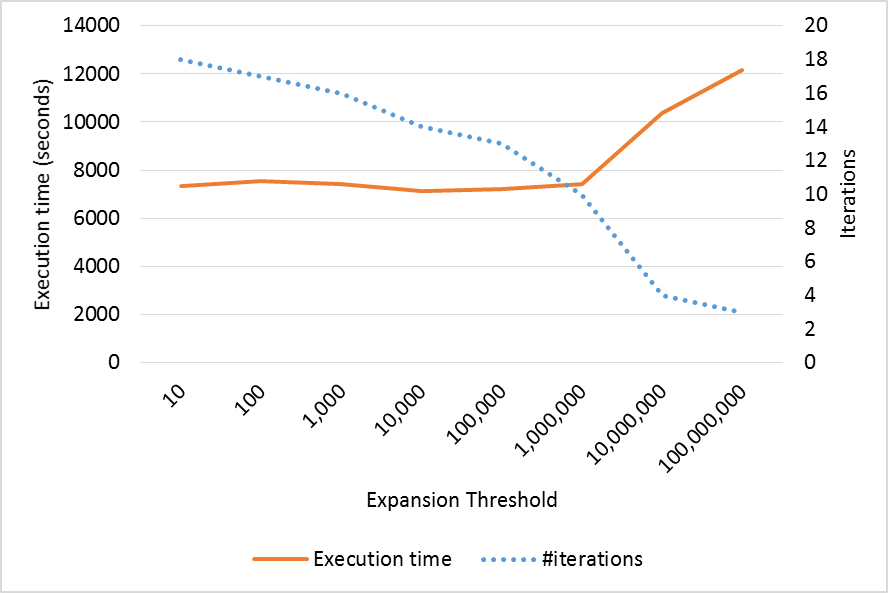
\includegraphics[width=5in]{immagini_extension/pems_fixed.png}
\caption{Execution time and number of iterations for different $max\_exp$ values on PEMS-SF dataset with $minsup$=10.
}
\label{pems_fixed}
\end{figure}

\begin{figure}[!t]
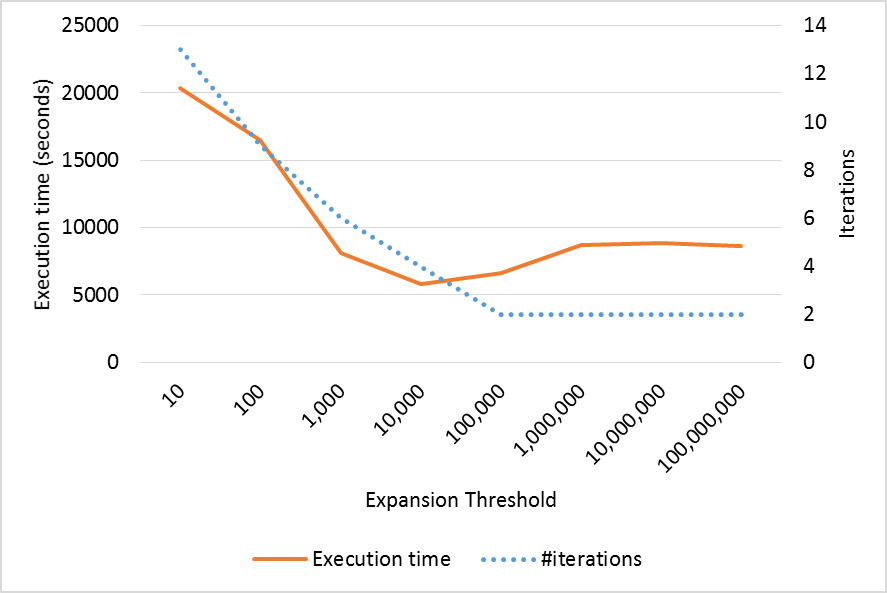
\includegraphics[width=5in]{immagini_extension/breast_fixed.png}
\caption{Execution time and number of iterations for different $max\_exp$ values on Breast Cancer dataset with $minsup$=5.
}
\label{breast_fixed}
\end{figure}

The same experiment is repeated with the Breast Cancer dataset and a minsup value of 5. As shown in Figure~\ref{breast_fixed}, even in this case, the best performances are achieved with $max\_exp$ equal to 10,000. In this case, differences are more significant with lower $max\_exp$ values, although with a non-negligible performance degradation with higher values. 

The value of $max\_exp$ impacts also the load balancing 
of the distributed computation among different nodes.
With low values of $max\_exp$, each task explores a
smaller enumeration sub-tree, decreasing the size difference
among the sub-trees analyzed by different tasks,
thus improving the load balancing.
Table~\ref{load balance breast} reports the minimum and the maximum execution time of
the mining tasks executed in parallel for both the datasets and for two extreme values of $max\_exp$. 
The load balance is better for the lowest value of $max\_exp$.



\begin{table}
\begin{center}
\caption{Load Balancing}
\label{load balance breast}
\begin{tabular}{ |c| c | c| c| c| }
\hline
							    &
\multicolumn{2}{|c|}{Task execution time}    & \multicolumn{2}{|c|}{Task execution time}      \\ 
 & \multicolumn{2}{|c|}{Breast Cancer}    & \multicolumn{2}{|c|}{PEMS-SF}      \\ \hline \hline
	Maximum expansion threshold &   Min          & Max    &   Min          & Max          \\ \hline
	100,000,000                 &    7 m                      & 2h 16m 17s &    44s                      & 2h 20m 28s
  \\ \hline
10                         &    6m 21s                      &        45m 16s  &   6s                      &        2m 24s
 \\ \hline
\end{tabular}
\end{center}
\end{table}





The $max\_exp$ choice has a non-negligible impact on the performances of the algorithm. However, as demonstrated by the curves in Figures~\ref{pems_fixed} and~\ref{breast_fixed}, it is very dependent on the use case and distribution of the data.
In the next subsection we introduce and motivate some tuning strategies related to $max\_exp$.

%
%This set of experiments has been performed on the Breast cancer dataset
%with Minsup 5, by varying $max\_exp$ from 100 to 100,000,000. This minsup value allowed to notice different
%wall-clock time for each expansion threshold value.
%Figure~\ref{exp_1} shows the results in terms of execution time and number of iterations 
%(i.e., the number of jobs).
%The best performance in terms of execution time is achieved with a maximum
%expansion threshold equal to 10,000 nodes.
%With higher values, the number of iterations decreases,
%but more useless tree branches are explored,
%because pruning rule 3 is globally applied less frequently.
%Lower values of  $max\_exp$, instead, introduce a performance
%degradation caused by the higher number of iterations
%and the synchronization phase overheads.
%With very high values of  $max\_exp$, the running time and the number of
%iterations are stable because the bottleneck becomes the free available
%memory, and the synchronization job is
%automatically applied, independently of the value of  $max\_exp$.
%The tuning of $max\_exp$ is strictly related to the data distribution:
%in general, the easier the mining task, the fewer the benefits of having 
%many iterations.
%
%The value of $max\_exp$ impacts also the load balancing 
%of the distributed computation among different nodes.
%With low values of $max\_exp$, each task explores a
%smaller enumeration sub-tree, decreasing the size difference
%among the sub-trees analyzed by different tasks,
%thus improving the load balancing.
%Table~\ref{load balance} reports the minimum and the maximum execution time of
%the mining tasks executed in parallel for two extreme values of $max\_exp$. 
%The load balance is better for the lowest value of $max\_exp$.
%\textbf{tutto vecchio fin qui}
%
%
%\begin{figure}[!t]
%\includegraphics[width=5in]{grafo_exp2.png}
%\caption{Execution time and number of iterations for different $max\_exp$ values on Breast Cancer dataset with $minsup$=5.
%}
%\label{exp_1}
%\end{figure}
%
%
%\begin{table}
%\begin{center}
%\caption{Load Balancing}
%\label{load balance}
%\begin{tabular}{ |c| c | c| }
%\hline
%							    &
%\multicolumn{2}{|c|}{Task execution time}          \\ \hline
%	Maximum expansion threshold &   Min          & Max            \\ \hline
%	100,000,000                 &    4s                      & 1h 54m 33s
%  \\ \hline
%100,000                 &    4s                      & 1h 2m 32s
%  \\ \hline
%	10000                         &    4s                      &        23m 50s
%\\ \hline
%100                         &    4s                      &        53s
% \\ \hline
%\end{tabular}
%\end{center}
%\end{table}


\subsection{Proposed strategies}\label{exp_strategies}
This section introduces some heuristic strategies related to the $max\_exp$ parameter. 
The aim of this experiment is to identify an heuristic technique which is able to deliver good performances without the need by the user to tune up the the $max\_exp$ parameter.
Before the introduction of the techniques, let us motivate the reasons behind their design.
Because of the enumeration tree architecture, the first tables of the tree are the most populated. Each node, in fact, is generated from its parent node as a projection of the parent transposed table on a tid. 
In addition, the first nodes are, in the average, the ones generating more sub-branches. By construction, their transposed table tidlists are, by definition, longer than the ones of their children nodes. This increases the probability that the table could be projected on a tid.
For these reasons, the tables of the initial mining phase are the most heavy to be processed.
On the other hand, the number of nodes to process by each local Carpenter iteration tends to increase with the number of iterations. Still, this factor is mitigated by (i) the decreasing size of the tables and (ii) the eventual end of some branches expansion (i.e. when there are not more tids in the node transposed table).
These reasons motivated us to introduce some strategies that assume a maximum expansion threshold that is increased with the number of iterations. These strategies start with very low values in very initial iterations  (i.e. when the nodes are more heavy to be processed) and increase $max\_exp$ during the mining phases.

The strategy \#1 is the most simple: the $max\_exp$ is increased with a factor of $X$ at each iteration. For instance, if the $max\_exp$ is set to 10, and $X$ is set to 100 at the second iteration it is raised to 1000 and so on.
In addition to this straightforward approach, we have tried to leverage informations about the execution time of each iteration and the pruning effect (i.e. the percentage of transposed tables / nodes that are pruned in the synchronization job). 
Specifically, strategy \#2 consists in increasing, at each iteration, the $max\_exp$ parameter with a factor of  $X^{T_{old} / T_{new}}$, given $T_{new}$ and  $T_{old}$ the execution time of the previous two jobs. The motivation is to balance the growth of the parameter in order to achieve a stable execution times among the iterations.  
For strategy \#3, we take into account the relative number of pruned tables. Indeed, this value cannot be easily interpreted. An increasing pruning percentage means that there are a lot of tables that are generated uselessly. However, an increasing trend is also normal, since the number of nodes that are processed increases exponentially. Given that our intuition is to rise the  $max\_exp$ among the iterations, in strategy \#3, we increase the $max\_exp$ parameter with a factor $X^{Pr_{old} / Pr_{new}}$, given $Pr_{new}$ and  $Pr_{old}$ the relative number of pruned tables in the previous two jobs. 
Finally, strategy \#4 is inspired by the congestion control of TCP/IP (a data transmission protocol used by many Internet applications~\cite{Jacobson:1988:CAC:52325.52356}). Precisely, the $max\_exp$ is handled like the congestion window size (i.e. the number of packets that are sent without congestion issues).
This strategy, called ``Slow Start'', assumes two types of growing of the window size: an exponential one and a linear one. In the first phase, the window size is increased exponentially until it reaches a threshold (``ssthresh'', which is calculated from some empirical parameters such as Round Trip Time value). From that moment, the growth of the window becomes linear, until a data loss occurs.
In our case, we just inherit the two growth factor approach. Therefore, our ``slow start'' strategy consists in increasing the $max\_exp$ of a factor of $X$ until the last iteration reaches an execution time greater than a given threshold. After that, the growth is more stable, increasing the parameter of a factor of 10 (for this reason $X\geq10$).
We have fixed the threshold to the execution time of the first two jobs (Job 1 and Job 2). These jobs, for the architecture of our algorithm, consists of the very first Carpenter iteration. They are quite different than the others since the first Mapper phase has to build the initial projected transposed tables (first level of the tree) from the input file. This choice is consistent with our initial aim, that is to normalize the execution times of the last iterations which are often shorter than the first ones.
\textbf{Fabio \& Paolo:Non siamo sicuri che convenga inserire questa parte sul time out. Michiardi: I guess it is ok: mechanisms like speculative execution work similarly, hence to me the approach is not shocking}.
The increasing $max\_exp$ value introduced by the described strategies, however, leads to a degradation of the load balancing between the parallel tasks of the job. To limit this issue, we have introduced a timeout of 1 hour. After that, all the tasks will be forced to run the synchronization job. From the algorithmic point of view, this is not a loss, since the the tables are expanded in a depth-first fashion. The last tables, hence, are the ones with the highest probability to be pruned. Although, in this way, we are limiting to 1 hour the amount of time in which we are not completely exploiting the resources of the commodity cluster (i.e. only few very long tasks running). A value of 1 hour has been empirically proved to be a good trade-of between load balancing and a good leveraging of the centralized memory pruning.

\begin{table}
\begin{center}
\caption{Strategies}
\label{table_strategies}
\begin{tabular}{|c|c|}
\hline
Strategy \#1($X$)  & Increasing at each iteration      \\ 
                   & with a factor of $X$               \\ \hline

Strategy \#2($X$)  & Increasing at each iteration with \\
                   & a factor of $X^{T_{old} / T_{new}}$                   \\ \hline


Strategy \#3($X$) & Increasing at each iteration with \\
                   & a factor of $X^{Pr_{old} / Pr_{new}}$                    \\ \hline
                   Strategy \#4       & Slow start, with a fast increase                      \\ 
     & factor of   $X$                     \\ \hline
            
\end{tabular}
\end{center}
\end{table}


\begin{table}
\begin{center}
\caption{Strategies performance}
\label{strategies_perf}
\begin{tabular}{ |c| c | c| }
\hline
 Strategies & PEMS-SF& Breast Cancer   \\ \hline \hline
  Strategy \#1 &-6.48 \%   &    -19.03 \\ 
   &
 (X = 10)  &   (X = 100,000 )   \\ \hline
  Strategy \#2 & --3,73\% &  -0.02 \%   \\ 
      & (X = 1,000)&  (X = 10,000 )    \\ \hline
  Strategy \#3 & -4,42
 \%  & +1.59 \%   \\ 
      &  (X = 100)&  (X = 100)   \\ \hline
   Strategy \#4 & +9,39
 \%
 &  -16.17 \%   \\ 
      &(X = 100) & (X = 1,000 )    \\ \hline
\end{tabular}
\end{center}
\end{table}

Strategy \#1 is the one achieving the best performances for both the datasets. In Table~\ref{strategies_perf} are resumed the best performance for each strategy, in terms of relative performance difference with the best results obtained with a fixed $max\_exp$ parameter. For PEMS-SF dataset, even strategies \#2 and \#3 are able to achieve positive gains. For Breast Cancer dataset strategy \#1 is the best, followed by strategy \#4: these are the only ones achieving significant positive gain over the fixed $max\_exp$ approach.
All the strategies are evaluated with $X$ from 10 to 10,000. The max value has been increased in the cases in which the performance suggest a decreasing execution time trend.

Since the best performance is achieved with values of 10 and 100,000 respectively for PEMS-SF and Breast Cancer datasets (Figures~\ref{pems_strategy1} and~\ref{breast_strategy1}), we will use this configuration for the experiments comparing PaMPa-HD with other distributed approaches. \textbf{(queste figure sono indispensabili?) Michiardi: in my opinion either: i) we omit them and only report \# in the text ii) we put a table}The difference may be caused by the characteristics of the dataset: evidently, PEMS-SF dataset benefits of more synchronization phases.


%Finally, in all the experiments \textbf{citare quelli di prima}, we have notices some very short execution times (less than a minute) in the last mining iterations. This surely increases the impact of MapReduce job handling overhead on the global performances.
%All these things, motivated us to introduce some strategies that assumes a maximum expansion threshold that is increased with the number of iterations.
%All these things, together with very short last iterations (with an increasing MapReduce job overhead), motivated us to test some strategies that assumes a maximum expansion threshold that is increased with the iterations.

%The strategy \#1 is straightforward: the $max\_exp$ is increased with a factor of $X$ at each iteration. For instance, if the $max\_exp$ is set to 10, and $X$ is set to 100 at the second iteration it is raised to 1000 and so on. 
%
%Alternatively, we wanted to achieve a balanced growth of the $max\_exp$ parameter. We want to balance the load of the iterations, but, on the other hand, we want to avoid an overgrowth of the parameter and, therefore, of the execution times of the last iterations. As already said, in fact, increasing the $max\_exp$ parameter decreases the impact of the synchronization job pruning.
%In order to monintor the growth, we introduced a set of techniques based on the execution times and a strategy which monitors the impact of the synchronization jobs.
%%In order to monitor this growth, we firstly thought about an index measuring the effectiveness of the pruning in terms of closed or tables pruned in the synchronization job. However, the effectiveness of the pruning cannot be easily interpreted. An increasing pruning effect means that there are a lot of tables that are generated uselessly. However, an increasing pruning effect is also normal since the number of nodes that are processed continues to increase. \textbf{inserire degli esperimenti in cui faccio vedere che usare il pruning effect riduce le performance}.
%In strategies \#2 and \#3, we took into exam the execution time of the iterations.
%Spefically, strategy \#2 consists in increasing, at each iteration, the $max\_exp$ parameter with a factor of  $X^{T_{old} / T_{new}}$, given $T_{new}$ and  $T_{old}$ the execution time of the previous two jobs. The motivation is to balance the growth of the parameter in order to achieve a stable execution times among the iterations.  
%Strategy \#3, instead, is inspired by the congestion control of TCP/IP (a data transmission protocol used by many Internet applications~\cite{}). Precisely, the $max\_exp$ is handled like the congestion window size (i.e. the number of packets that are sent without congestion issues).
%This strategy, called ``Slow Start'', assumes two types of growing of the window size: an exponential one and a linear one. In the first phase, the window size is increased exponentially until it reaches a threshold (``ssthresh'', which is calculated empirically from RTT and other values). From that moment, the growth of the window becomes linear, until a data loss occurs.
%In our case, we are not interested we just inherit the two growth factors. Therefore, our ``slow start'' strategy consists in increasing the $max\_exp$ of a factor of $X$ until the last iteration reaches an execution time greater than a given threshold. After that, the growth is more stable, increasing the parameter of a factor of 10 (for this reason $X$>10).
%We have fixed the threshold to the execution time of the first two jobs (Job 1 and Job 2). These jobs, for the architecture of our algorithm, consists of the very first Carpenter iteration. They are quite different than the others since the first Mapper phase has to build the initial projected transposed tables (first level of the tree) from the input file. 
%We have selected the execution time of the first iteration since it is consistent with our initial aim,
%that is to normalize the execution times of the last iterations which are often shorter than the first ones.
%
%The last strategy, \#4, is based on the effectiveness of the pruning in terms of closed or tables pruned in the synchronization job. Indeed, the measure of the relative number of tables that are pruned cannot be easily interpreted. An increasing pruning percentage means that there are a lot of tables that are generated uselessly. However, an increasing trend is also normal, since the number of nodes that are processed continues to increases. Given that our intuition is to rise the  $max\_exp$ among the iterations, in strategy \#4, we increase the $max\_exp$ parameter with a factor $X^{Pr_{old} / Pr_{new}}$, given $Pr_{new}$ and  $Pr_{old}$ the relative number of pruned tables in the previous two jobs. 
%%Even if strategy \#4 can be meant as the dual of strategy \#2, with the usage of the pruning ratios instead of the different execution times, we decided not to do the same for strategy \#3. In this case, we could not identify a proper threshold to be used for changing the growth factor of $max\_exp$. In strategy \#3, we have used the first iteration because the initial motivation of this empirical study is to stabilize the execution times. In this case, we don't consider the initial pruning ratio as a valid threshold: it is computed after only few tables and, in the worst case, can be 0.
%
%In our experiment, we have fixed the initial  $max\_exp$ value to 10. This very low value is motivated by the nature of our strategies, which consist of a balanced increasing of the parameter.
%We applied the strategies (resumed in Table~\ref{table_strategies}) to the same experiments of Figures~\ref{breast_fixed} and ~\ref{pems_fixed}, in order to compare execution times the ones obtained with the optimum choice of $max\_exp$. 
%In oder to assess the impact of the $X$ parameter, we have used values from 10 to 10,000 (except for strategy3 for which we have used values from 100 to 10,000).
%
%The result of the application of the techniques to the PEMS-SF dataset are shown in Figures~\ref{pems_strategy1},~\ref{pems_strategy2},~\ref{pems_strategy3},~\ref{pems_strategy4}, which represent the relative execution time gain with respect to the best execution time obtained with the fixed $max\_exp$ of 10,000. In Figure~\ref{pems_strategy_best} we have grouped the best configuration for each strategy in order to easily compare them.
%It is clear how the almost all the strategies improve the performance of the algorithm. Only Strategy3 showed to be slower. Strategy1(1,000), Strategy2(10,000) and Strategy4(1,000) achieve a very similar speedup. 
%
%We have repeated the experiment with Breast Cancer dataset and a minsup value of 6 (Figures~\ref{breast_strategy1},~\ref{breast_strategy2},~\ref{breast_strategy3},~\ref{breast_strategy4}). We have raised $X$ from 10 to 10,000. Only with Strategy2, as shown in Figure~\ref{breast_strategy2}, we have raised it to 100,000 , because the experiments could suggest a decreasing execution times trend, but it was not the case.
%As before, the results are grouped in Figure~\ref{breast_strategy_best}.
%In this case, all the strategies achieve a positive speedup with respect to the best execution time obtained with a fixed $max\_exp$ parameter. In addition, the same configurations for each strategy demonstrated to be most performant in both the experiments.
%The results obtained with the adoption of these strategies are very similar, and the differences are negligible.
%
%
%

\begin{figure}[!t]
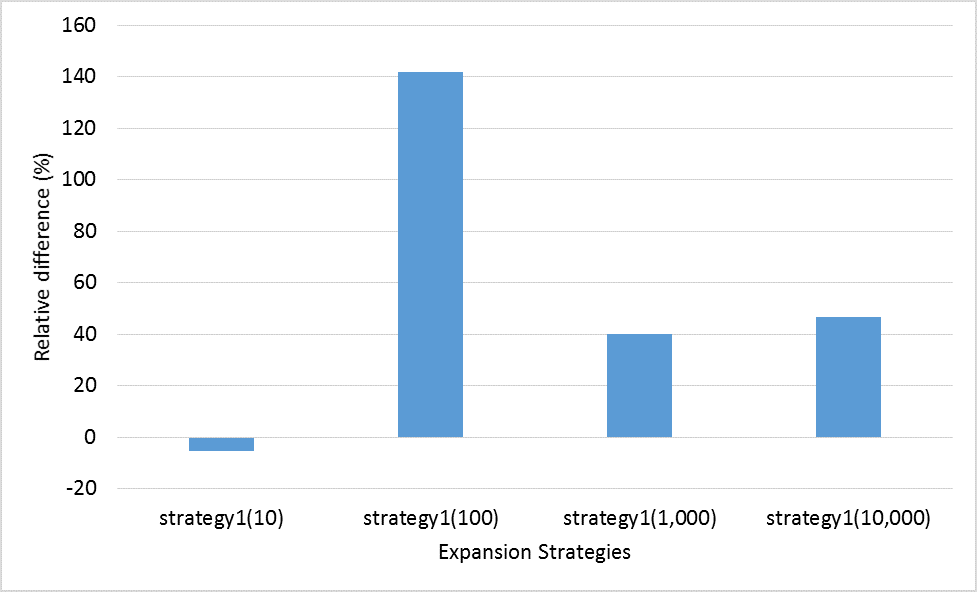
\includegraphics[width=5in]{immagini_extension/pems_strategy1.png}
\caption{Relative gains on Pems-SF dataset with $minsup$=10, Strategy1 and different $X$ values.
}
\label{pems_strategy1}
\end{figure}

%\begin{figure}[!t]
%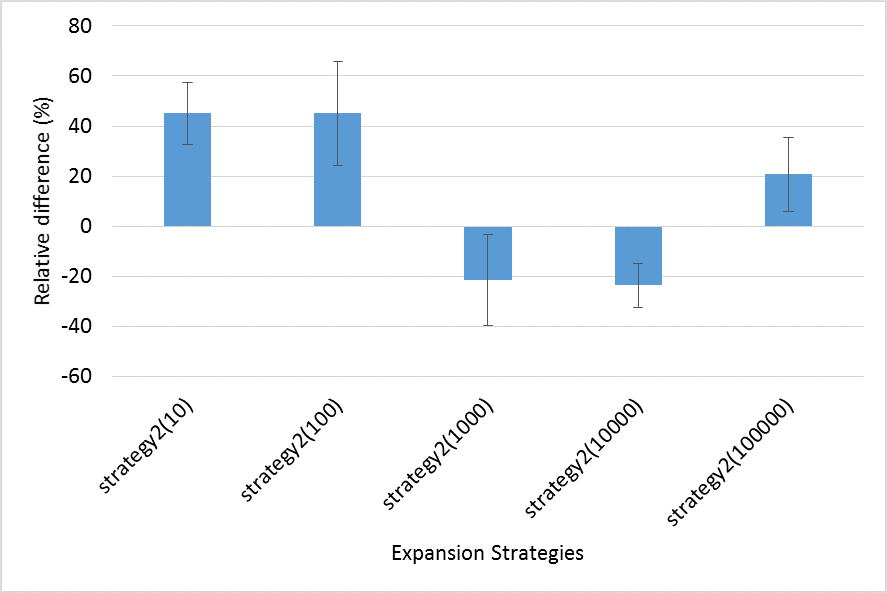
\includegraphics[width=5in]{immagini_extension/pems_strategy2.png}
%\caption{Relative gains on Pems-SF dataset with $minsup$=50, Strategy2 and different $X$ values.
%}
%\label{pems_strategy2}
%\end{figure}
%
%\begin{figure}[!t]
%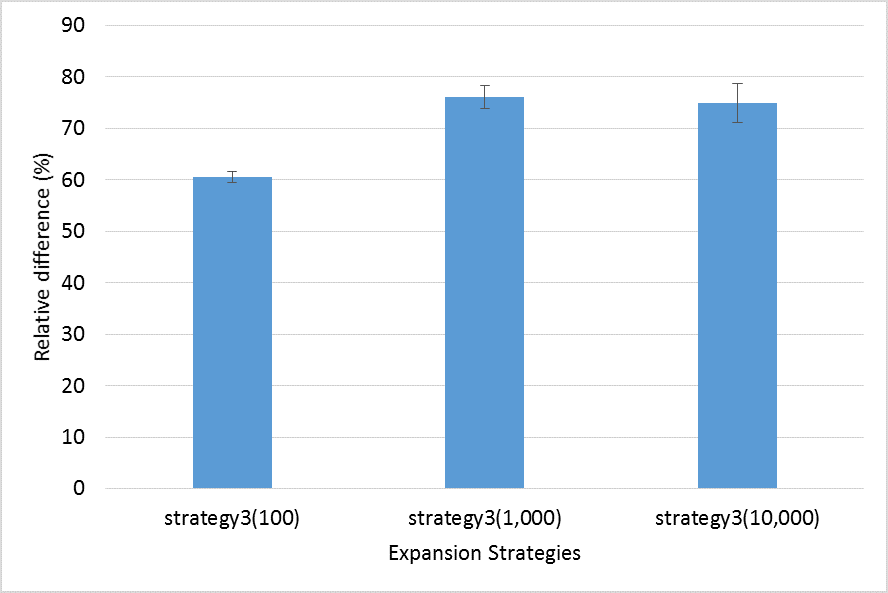
\includegraphics[width=5in]{immagini_extension/pems_strategy3.png}
%\caption{Relative gains on Pems-SF dataset with $minsup$=50, Strategy3 and different $X$ values.
%}
%\label{pems_strategy3}
%\end{figure}
%
%\begin{figure}[!t]
%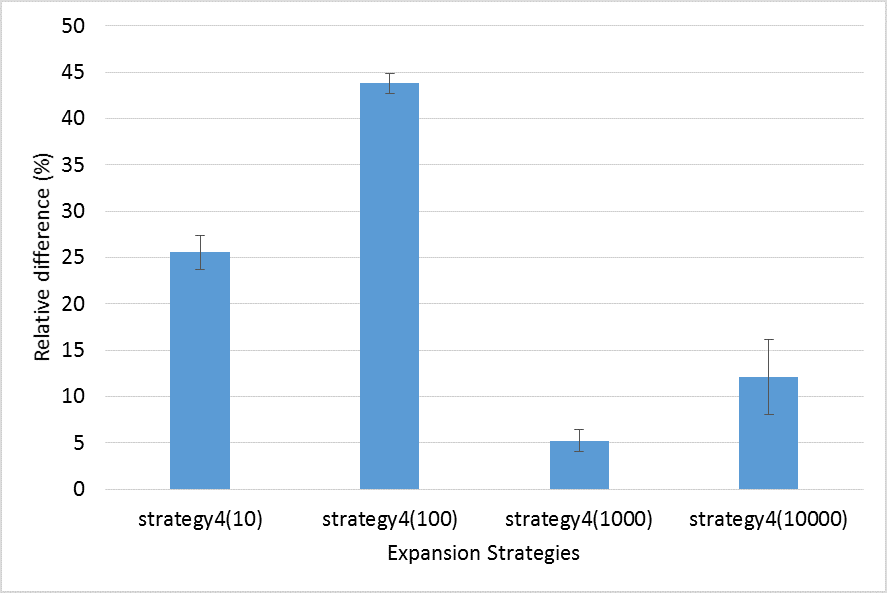
\includegraphics[width=5in]{immagini_extension/pems_strategy4.png}
%\caption{Relative gains on Pems-SF dataset with $minsup$=50, Strategy4 and different $X$ values.
%}
%\label{pems_strategy4}
%\end{figure}
%
%\begin{figure}[!t]
%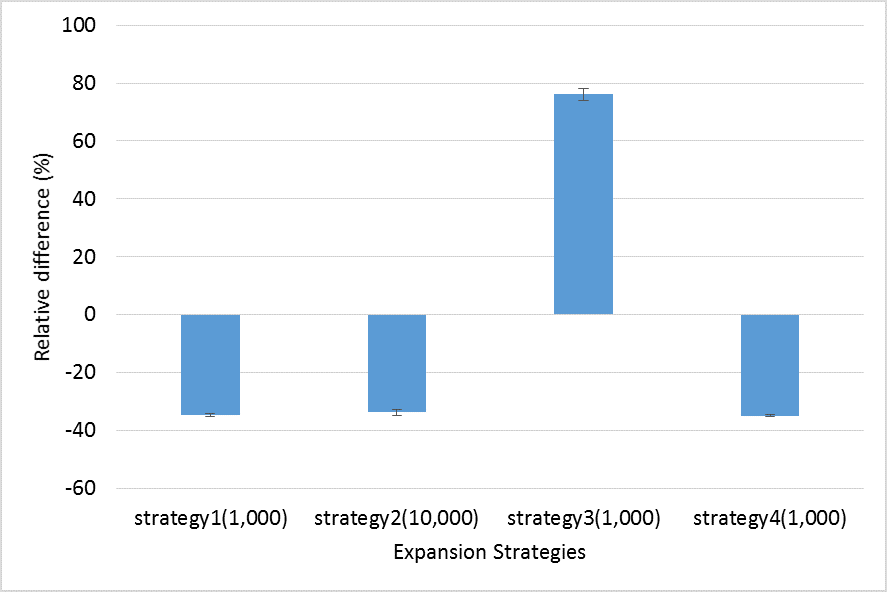
\includegraphics[width=5in]{immagini_extension/pems_strategy_best.png}
%\caption{Relative gains of the best configuration for each strategy, on Pems-SF dataset with $minsup$=50.
%}
%\label{pems_strategy_best}
%\end{figure}
%
%
\begin{figure}[!t]
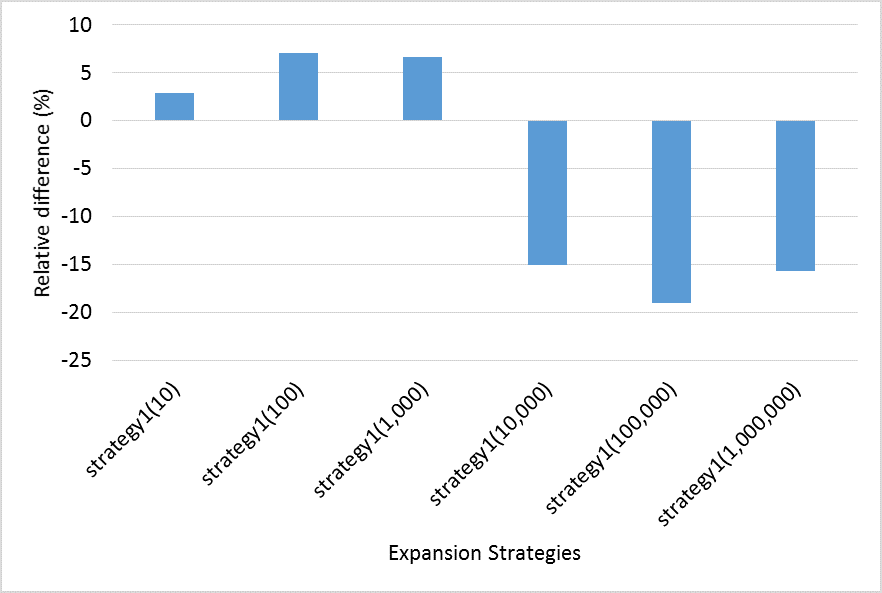
\includegraphics[width=5in]{immagini_extension/breast_strategy1.png}
\caption{Relative gains on Breast Cancer dataset with $minsup$=5, Strategy1 and different $X$ values.
}
\label{breast_strategy1}
\end{figure}

%\begin{figure}[!t]
%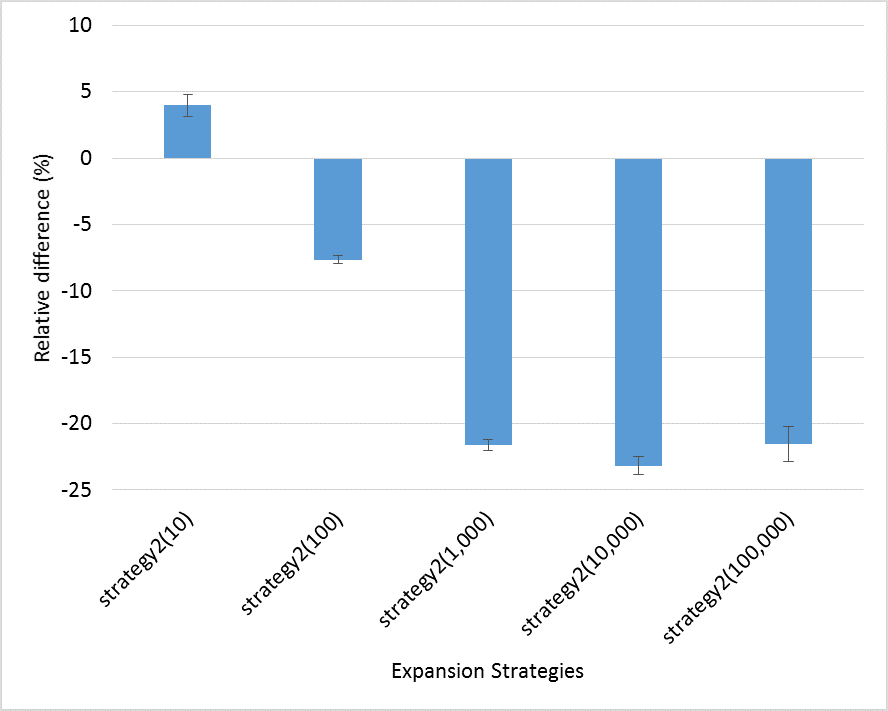
\includegraphics[width=5in]{immagini_extension/breast_strategy2.png}
%\caption{Relative gains on Breast Cancer dataset with $minsup$=6, Strategy2 and different $X$ values.
%}
%\label{breast_strategy2}
%\end{figure}
%
%\begin{figure}[!t]
%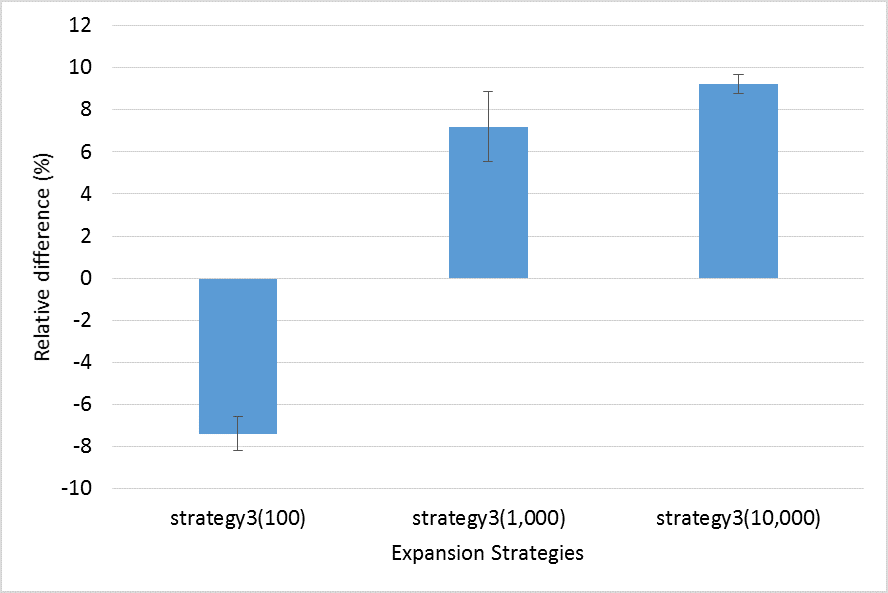
\includegraphics[width=5in]{immagini_extension/breast_strategy3.png}
%\caption{Relative gains on Breast Cancer dataset with $minsup$=6, Strategy3 and different $X$ values.
%}
%\label{breast_strategy3}
%\end{figure}
%
%\begin{figure}[!t]
%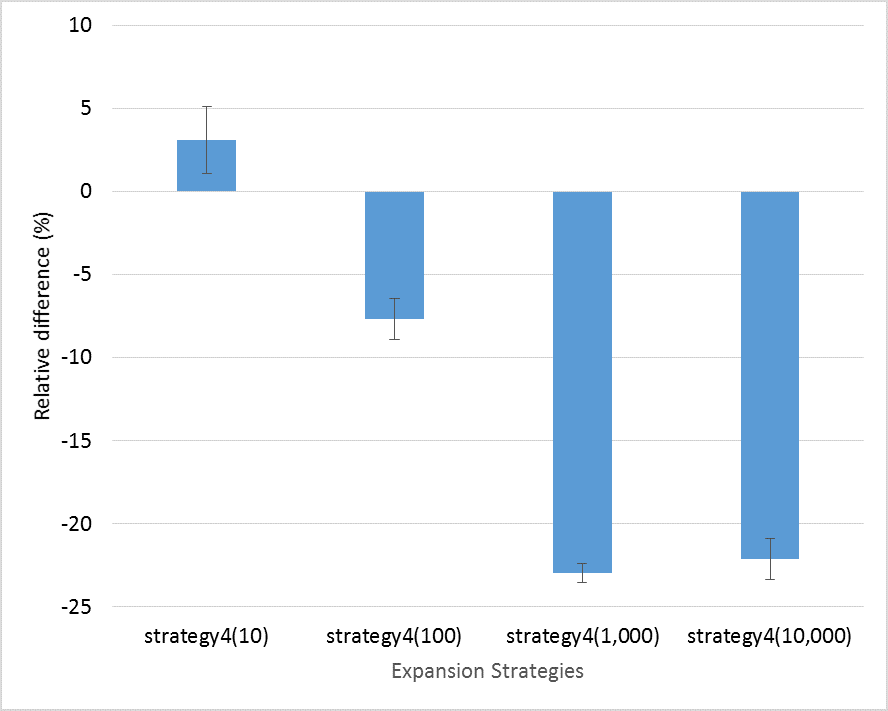
\includegraphics[width=5in]{immagini_extension/breast_strategy4.png}
%\caption{Relative gains on Breast Cancer dataset with $minsup$=6, Strategy4 and different $X$ values.
%}
%\label{breast_strategy4}
%\end{figure}
%
%\begin{figure}[!t]
%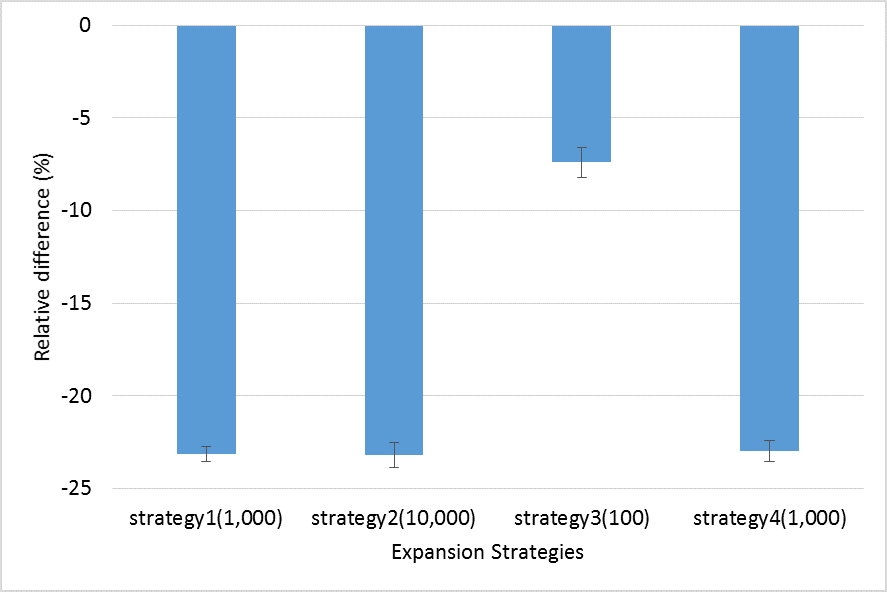
\includegraphics[width=5in]{immagini_extension/breast_strategy_best.png}
%\caption{Relative gains of the best configuration for each strategy, on Pems Cancer dataset with $minsup$=6.
%}
%\label{breast_strategy_best}
%\end{figure}
%


\subsection{Running time}\label{running_time}
After the identification of a good trade-of strategy in the previous section, we have used it to analyze the efficiency of PaMPa-HD
comparing it with three distributed state-of-the-art frequent itemset mining algorithms:
\begin{enumerate}
\item Parallel FP-growth~\cite{pfpgrowth} available in Mahout 0.9~\cite{Mahout}, based on FP-Growth algorithm~\cite{Han00}

\item DistEclat~\cite{bigfim}, based on Eclat algorithm~\cite{Zaki97newalgorithms}
\item BigFIM~\cite{bigfim}, inspired from Apriori~\cite{Agr94} and DistEclat
\end{enumerate}
This set of algorithms represents the most cited implementation of frequent itemset mining distributed algorithms. All of them are Hadoop-based and are designed to extract the frequent closed itemsets (DistEclat and BigFIM actually extract a superset of the frequent closed itemsets).
The parallel implementation of these algorithms has been aimed to scale in the number of transactions of the input dataset. Therefore, they are not specifically developed to deal with
high-dimensional datasets as PaMPa-HD. 
For details about the algorithms, see Section~\ref{Related work}.

%The comparison with Carpenter aims to show the ability of PaMPa-HD
%to address datasets that are not manageable by means of a
%centralized approach.
%The comparison with the Hadoop implementation of PFP is
%a reference benchmark since it represents
%the most scalable state-of-the-art approach for closed itemset
%mining, even if PFP was not specifically developed to deal with
%high-dimensional datasets as PaMPa-HD.
The first set of experiments has been performed with the 100-rows version PEMS-SF dataset~\cite{uci} and minsup values 35 to 5.\footnote{The algorithms parameters, which will be introduced in Section~\ref{Related work}, has been set in the following manner. PFP has been set to obtain all the closed itemsets; the prefix length of the first phase of BigFIM and DistEclat, instead, has been set to 3, as suggested by the original paper~\cite{bigfim}, when possible (i.e. when there were enough 3-itemsets to execute also the second phase of the mining).}

As shown in Figure~\ref{pems_confronto}, in which minsup axis is reversed to improve readability, PaMPa-HD is the only algorithm able to complete all the mining task to a minsup value of 5 rows or 5\%. All the approaches show similar behaviors with high minsup values (from 30 to 35).
With a minsup of 25, PFP shows a strong performance degradation, being not able to complete the mining.
In a similar way, BigFIM shows a performance degradation with a minsup of 20, running out of memory with a minsup of 15. 
DistEclat, instead, shows very interesting execution time until running out of memory with a minsup of 10.
PaMPa-HD, even if slower than DistEclat with minsup values from 25 to 15, is able to complete all the tasks.


\begin{figure}[!t]
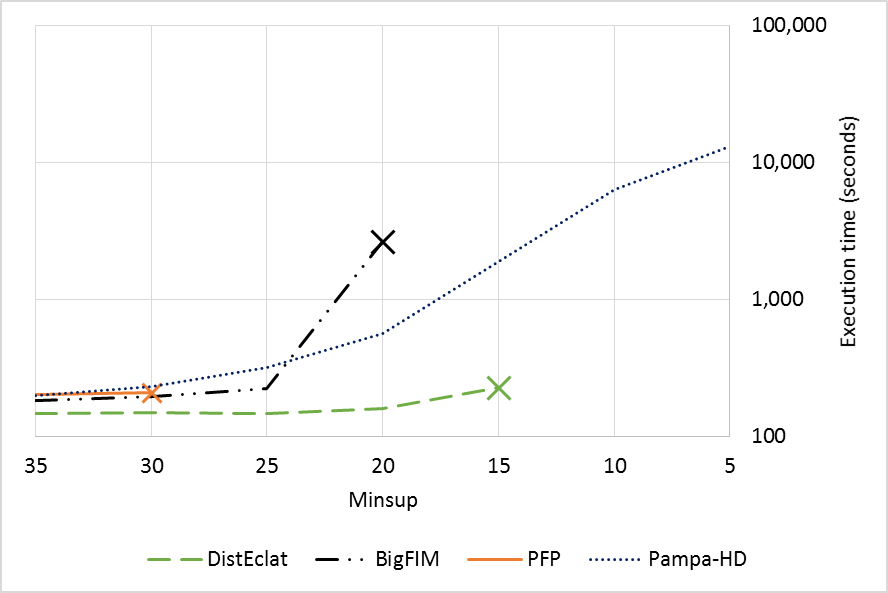
\includegraphics[width=5in]{immagini_extension/pems_confronto.png}
\caption{Execution time for different Minsup values on the PEMS-SF dataset (100-rows).}
\label{pems_confronto}
\end{figure}

\begin{figure}[!t]
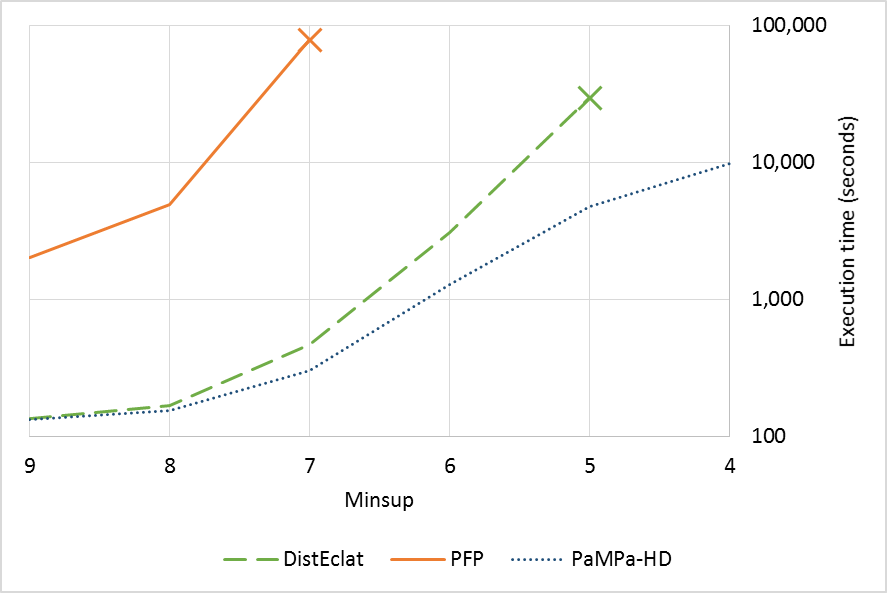
\includegraphics[width=5in]{immagini_extension/breast_confronto.png}
\caption{Execution time for different Minsup values on the Breast Cancer dataset.}
\label{breast_confronto}
\end{figure}
The second set of experiments are performed with the Breast
Cancer dataset~\cite{breast_cancer_dataset}.
As reported in Figure~\ref{breast_confronto} (Even in this case, minsup axis is reversed to improve readability, the minsup is absolute), PaMPa-HD is the most reliable and fast approach.
This time, BigFIM is not able to cope either with the highest minsup values, while PFP shows very slow execution times and runs out of memory with a minsup value of 6.
DistEclat is able to achieve good performances but it is always slower than PaMPA-HD (with a minsup value equal to 4, it is not able to complete the mining within several days of computation).
From these results, we have seen how  traditional best-in-class approaches such as BigFIM, DistEclat and PFP are not suitable for high-dimensional datasets. They are slow and/or not reliable when coping with the curse of dimensionality. PaMPa-HD, instead, demonstrated to be most suitable approach with datasets characterized by a high number of items and a small number of rows.
After the comparison with the state of the art distributed frequent itemset mining algorithm, the next experimental subsections will experimentally describe the behavior of PaMPa-HD with respect to the number of transactions, number of independent tasks, communication costs and load balancing.
%Because of the algorithm design of our approach, we already know that it is very sensitive with respect to the transactions of the input dataset. It will be interesting to evaluate the impact of the number of independent tasks. This issue is not trivial because adding a task to the computation would not only delivers more resources such as memory or CPU. An additional task leads to split the chunk of the enumeration tree that is explored

%\begin{figure}[!t]
%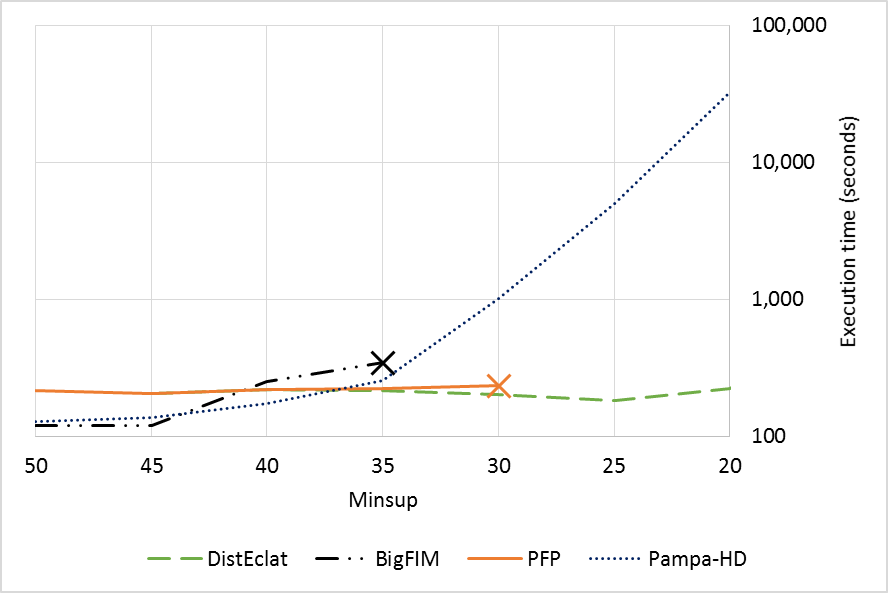
\includegraphics[width=5in]{immagini_extension/pems_confronto_200.png}
%\caption{Execution time for different Minsup values on the PEMS-SF dataset (200-rows).}
%\label{pems_confronto_200}
%\end{figure}

\subsection{Impact of the number of transactions}\label{number_rows}
This set of experiments measures the impact of the number of transactions on PaMPa-HD performances. At this aim, it will be used the PEMS-SF datasets in three versions (100-rows, 200-rows and full).
The algorithm is very sensitive to this factor: the reasons are related to its inner structure. In fact, the enumeration tree, for construction, is strongly affected by the number of rows. A higher number of rows leads to:
\begin{enumerate}
\item A higher number of branches. As shown in the example in Figure~\ref{running_1}, from the root of the tree, it is generated a new branch for each tid (transaction-id) of the dataset.
\item Longer and wider branches. Since each branch explores its research subspace in a depth-first order, exploring any combination of tids, each branch would result with a greater number of sub-levels (longer) and a greater number of sub-branches (wider)
\end{enumerate}

Therefore, the mining processes related to the 100-rows version and to the 200-rows or the full version of PEMS-SF dataset are strongly different. With a number of rows incremented by, respectively, 200\% and more of the 400\%, the mining of the augmented versions of PEMS-SF dataset is very challenging for the enumeration-tree based PaMPa-HD.
%The results in Figure~\ref{pems_confronto_200} and in Figuretoadd confirm these difficulties. With the same range of relative minsup values, BigFIM and PFP show a similar performance with the ones with the reduced version of the dataset (Figure~\ref{pems_confronto}). Their capacity to complete the mining is slightly and gradually reduced by some minsup values points.
%DistEclat, the algorithm which showed the most interesting performances among the ones not designed to fit high-dimensional use cases, shows a very stable behavior for all the mining tasks of the experiments in Figure~\ref{pems_confronto_200}. In the experiments with the full version of the dataset, interestingly, is not able to complete the mine even with a minsup of 50\%.
%PaMPa-HD shows a very strong performance degradation already in the experiments with 200-rows dataset, due to the higher number of transaction. Given $n$ the number of rows of the dataset, the size of the enumeration tree is proportional to $n^2$ \textbf{(che ne pensate?)} (while the approaches used by DistEclat, BigFIM and PFP are sensitive to the number of different items). 
The performance degradation is resumed in Figure~\ref{pampa_pems_confronto}, where, for instance, with a minsup of 35\%, the execution times related to the 100-rows and the full version of the PEMS-SF dataset differ of almost two orders of magnitude.

The behavior and the difficulties of PaMPa-HD with datasets with an incremental number of rows, is, unfortunately, predictable. This algorithmic problem represents a challenging and interesting open issues for further developments.
\begin{figure}[!t]
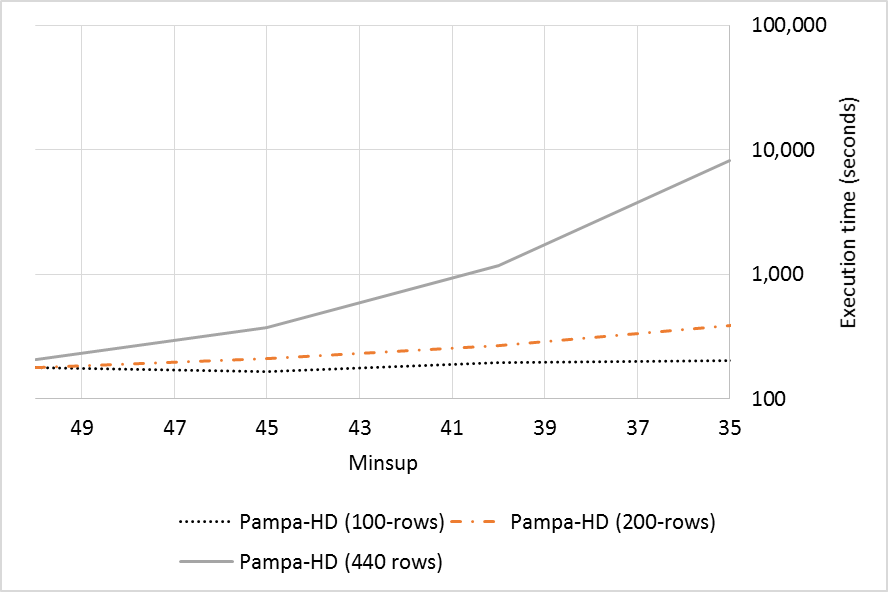
\includegraphics[width=5in]{immagini_extension/pampa_pems_confronto.png}
\caption{Execution times for different version of the PEMS-SF for PaMPa-HD.}
\label{pampa_pems_confronto}
\end{figure}
%The Hadoop PFP implementation reveals to be unsuitable for the
%extraction of frequent closed itemsets from the
%Kent Ridge Breast Cancer dataset:
%its execution time was more than one day of computation,
%even for the highest support threshold, 
%so orders of magnitude higher than the others.
%For this reason, the execution time of PFP is not reported in
%Figure~\ref{grafo_breast}. 
%BigFIM, instead, runs out of memory with XXX minsup values.
%These results highlight the need for specific algorithms
%particularly tailored to address high-dimensional data,
%such as PaMPa-HD,
%because traditional best-in-class approaches, such as PFP and DistEclat,
%cannot cope with the curse of dimensionality.

%
%\begin{figure}[!t]
%\includegraphics[width=5in]{grafo_breast.png}
%\caption{Execution time for different Minsup values on the Breast Cancer real dataset.}
%\label{grafo_breast}
%\end{figure}


%A second set of experiments using the synthetic Dataset~\#1 has been performed.
%In Dataset~\#1, even if the number of different items is only doubled 
%with respect to the breast cancer dataset, 
%the average number of items per transaction is much
%higher (one order of magnitude).
%This feature makes each conditional transposed table, associated with each node
%of the enumeration tree, much bigger and heavy to process.
%As reported in Figure~\ref{grafo_1}, 
%for very high Minsup values (20+) Carpenter scores the lowest execution times,
%with a Minsup value of 19 the performance of PaMPa-HD and Carpenter are almost the same,
%but with Minsup values of 18 or lower, Carpenter runs out of memory
%and the task is unfeasible, 
%whereas PaMPa-HD successfully completes the extraction.
%Furthermore, the time required for PaMPa-HD to complete the extraction in the latter case
%and its trend for decreasing Minsup values (19-18-17) 
%is equal or less than the time required by PFP 
%for respectively higher Minsup values (22-21-20).
%Not only PaMPa-HD is faster than PFP for high Minsup values (20+),
%but can it also scale further, since PFP stops at Minsup 20.
%The results prove that PaMPa-HD is effectively able to address problems 
%that are unfeasible for both centralized state-of-the-art specialized techniques (Carpenter)
%and scalable state-of-the-art generic itemset mining algorithms (PFP).
%
%
%%\begin{figure}[!t]
%%\includegraphics[width=5in]{grafo_dataset1.png}
%%\caption{Execution time for different Minsup values on synthetic Dataset~\#1.}
%%\label{grafo_1}
%%\end{figure}
%
%
%The last set of performance experiments is executed on synthetic Dataset~\#2.
%Dataset~\#2 is extremely high-dimensional, achieving an average number of
%items per transaction of 5,000,000.
%The results, reported in Figure~\ref{grafo_2}, confirm that 
%(i) for high Minsup values (21+), the problem is conveniently solved
%by current specialized algorithms (Carpenter),
%(ii) both centralized algorithms and generic distributed approaches
%cannot cope with high-dimensional datasets with lower Minsup values, 
%being 20 for Carpenter and 25 for PFP  the lowest feasible Minsup values,
%ad (iii) the proposed PaMPa-HD algorithm 
%provides both better execution times than PFP by almost an order of magnitude
%and higher scalability for more complex problems (lower Minsup values).
%Achieving lower Minsup values allows to discover deeply hidden knowledge, while high Minsup values usually lead to obvious information.
%%
%\begin{figure}[!t]
%\includegraphics[width=5in]{grafo_dataset2.png}
%\caption{Execution time for different Minsup values on synthetic Dataset~\#2.}
%\label{grafo_2}
%\end{figure}



%\subsection{Maximum expansion threshold}
%\label{impact_parameters}
%In this section we analyze the impact of the maximum expansion threshold
%($max\_exp$) parameter, which indicates the maximum number of nodes 
%to be explored before a preemptive stop of each distributed sub-process is forced.
%This parameter, as already discussed in Section~\ref{Distributed implementation outline},
%strongly affects the enumeration tree exploration,
%forcing each parallel task to stop before completing the visit of its sub-tree 
%and write partial results on HDFS. 
%This approach allows the synchronization job to globally apply 
%pruning rule 3 and reduce the search space.
%Low values of $max\_exp$ threshold decrease the risks of memory issue, 
%because the global problem is split into simpler and less memory-demanding
%sub-problems, and facilitate the application of pruning rule 3, 
%hence a smaller subspace is searched.
%However, higher values allow a more efficient execution,
%by limiting the start and stop of distributed tasks
%(similarly to the context switch penalty), and the synchronization overheads.
%
%
%This set of experiments has been performed on the Beast cancer dataset
%with Minsup 5, by varying $max\_exp$ from 100 to 100,000,000. 
%Figure~\ref{exp_1} shows the results in terms of execution time and number of iterations 
%(i.e., the number of times the synchronization Job \#2 is executed).
%The best performance in terms of execution time is achieved with a maximum
%expansion threshold equal to 10,000 nodes.
%With higher values, the number of iterations decreases,
%but more useless tree branches are explored,
%because pruning rule 3 is globally applied less frequently.
%Lower values of  $max\_exp$, instead, introduce a performance
%degradation caused by the higher number of iterations
%and the synchronization phase overheads.
%With very high values of  $max\_exp$, the running time and the number of
%iterations are stable because the bottleneck becomes the free available
%memory, and the synchronization job is
%automatically applied, independently of the value of  $max\_exp$.
%The tuning of $max\_exp$ is strictly related to the data distribution:
%in general, the easier the mining task, the fewer the benefits of having 
%many iterations.
%
%The value of $max\_exp$ impacts also the load balancing 
%of the distributed computation among different nodes.
%With low values of $max\_exp$, each task explores a
%smaller enumeration sub-tree, decreasing the size difference
%among the sub-trees analyzed by different tasks,
%thus improving the load balancing.
%Table~\ref{load balance} reports the minimum and the maximum execution time of
%the mining tasks executed in parallel for two extreme values of $max\_exp$. 
%The load balance is better for the lowest value of $max\_exp$.
%
%
%\begin{figure}[!t]
%\includegraphics[width=5in]{grafo_exp2.png}
%\caption{Execution time and number of iterations for different $max\_exp$ values on Breast Cancer dataset with $minsup$=5.
%}
%\label{exp_1}
%\end{figure}
%
%
%\begin{table}
%\begin{center}
%\caption{Load Balancing}
%\label{load balance}
%\begin{tabular}{ |c| c | c| }
%\hline
%							    &
%\multicolumn{2}{|c|}{Task execution time}          \\ \hline
%	Maximum expansion threshold &   Min          & Max            \\ \hline
%	100,000,000                 &    4s                      & 1h 54m 33s
%  \\ \hline
%100,000                 &    4s                      & 1h 2m 32s
%  \\ \hline
%	10000                         &    4s                      &        23m 50s
%\\ \hline
%100                         &    4s                      &        53s
% \\ \hline
%\end{tabular}
%\end{center}
%\end{table}




\subsection{Impact of the number of nodes}\label{scalability}
The impact of the number of independent tasks involved in the algorithm execution is not trivial issue. Adding a task to the computation would not only delivers more resources such as memory or CPU. An additional task leads to split the chunk of the enumeration tree that is explored by each task. On one hand, this means to reduce the search space to explore, lightening the task load. On the other hand, this reduces the state centralized memory and the impact of the related pruning. It can be interpreted as a trade-off between the benefits of the parallelism against the state. 
In Figure~\ref{scalability_img_pems} and Figure~\ref{scalability_img_breast}, it is reported the behavior of PaMPa-HD with a mining process on the datasets PEMS-SF and Breast Cancer. The minsup values, respectively of 20 and 6, have been chosen in order to be deep enough to show performance differences among the different degree of parallelism.
Interestingly, the mining on PEMS-SF dataset is less sensitive to the number of reducers, with an execution time that is just halved when the independent tasks included in the computation pass from 1 to 17. The experiment of Breast Cancer instead, Figure~\ref{scalability_img_breast}, shows a stronger performance gain. 
\textbf{(Lo stesso esperimento per quanto riguarda PEMS l'ho fatto con un minsup più basso e la linea era ancora più orizzontale}
The behavior is related to the dataset data distribution. 
For PEMS-SF dataset, the advantages related to additional independent nodes into the mining is mitigated by the loss from the point of view of state local pruning phase inside the nodes. With additional nodes, in fact, each node is pushed to a smaller exploration of the search space, decreasing the effectiveness of the local pruning.
%PEMS-SF dataset, as discussed in Subsection~\ref{exp_strategies}, mitigates the lack of additional independent nodes with a more aggressive local pruning phase inside the nodes.
These specific results recall a very popular open issue in distributed environment. In problems characterized by any kind of ''state'' benefit (in this case local pruning inside the tasks), a higher degree of parallelism does not lead to better performance a priori. \textbf{(Spero che si capisca, Michiardi mi aveva chiesto di riformulare)}
%\textbf{(Riformulare meglio, questo apre questioni interessanti sulla questione di determinare il grado di parallelismo quando si deve lanciare un algoritmo. Finora c'e' stato il forte constraint dei cluster fisici, ora col cloud tutti possono scegliere piu' liberamente. Quindi e' davvero vero che più grande e' il parallelismo migliori saranno le performance? Riprendere il tutto anche nelle conclusioni nelle open issues)}.

\begin{figure}[!t]
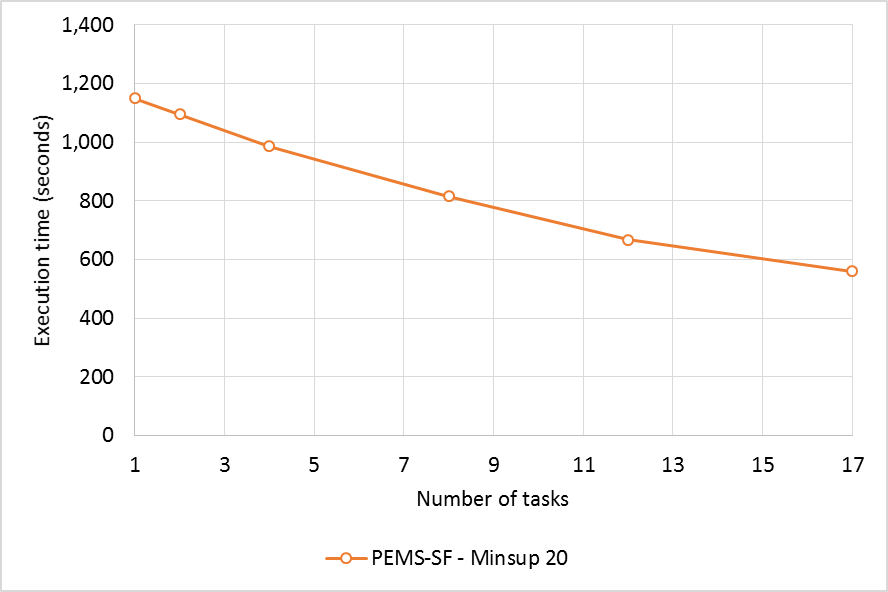
\includegraphics[width=5in]{immagini_extension/scalability_pems.png}
\caption{Execution times for PEMS-SF datasets with different number of parallel tasks.}
\label{scalability_img_pems}
\end{figure}

\begin{figure}[!t]
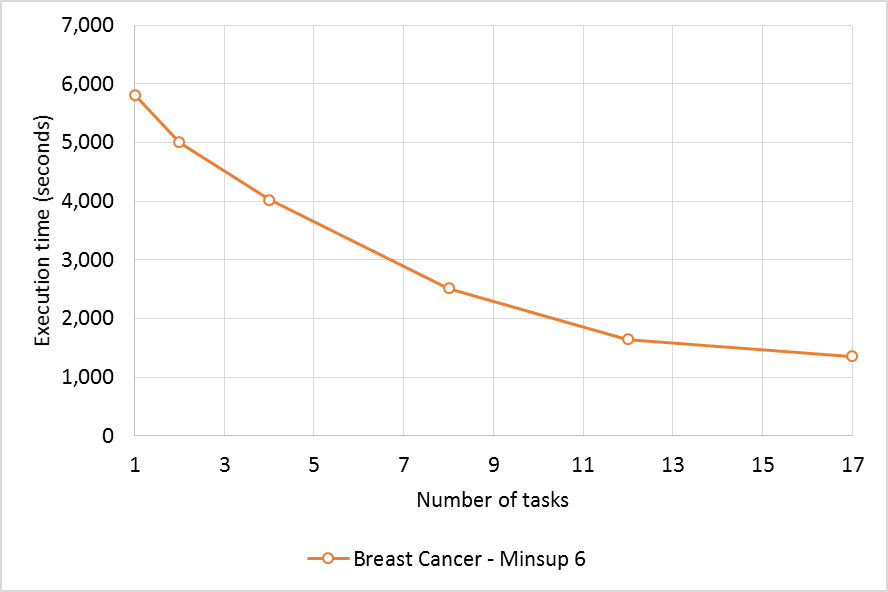
\includegraphics[width=5in]{immagini_extension/scalability_breast.png}
\caption{Execution times for Breast Cancer datasets with different number of parallel tasks.}
\label{scalability_img_breast}
\end{figure}


\subsection{Load Balancing and communication costs}\label{communication_cost}
The last analysis are related to the load balancing and the communication costs of the algorithm. These issues are very underestimated but they represent very important factor in such a distributed environment. Communication costs represent are among the main bottlenecks related to the performance of parallel  algorithms~\cite{Sarma:2013:ULB:2535570.2488334}. 
A bad-balanced load among the independent tasks leads to few long tasks that block the whole job.

PaMPa-HD, being based on Carpenter algorithm, as shown in the previous sections, mainly consists on the exploration of an enumeration tree. The basic idea behind the parallelization is to explore the main branches of the tree independently within parallel tasks (Figure~\ref{running_2}). For this reason, each task needs the information (i.e. transposed tables) related to its branch expansion. 
The ideal behavior of a distributed algorithm would be to distribute the least amount of data, avoiding redundant informations as much as possible. The reason is that network communications are very costly in a Big Data scenario.
Unfortunately, the structure of the enumeration tree of PaMPa-HD assumes that some pieces of data of the initial dataset is sent to more than one tasks. For instance, some data related to nodes $TT|_{2}$ and $TT|_{3}$ are the same, because from node $TT|_{2}$ will be generated the node $TT|_{2, 3}$. This is an issue related to the inner structure of the algorithm and a full independence of the initial data for each branch cannot be reached.

In addition, the architecture of the algorithm with its synchronization phase, burdens of the I/O costs. In fact, in order to prune some useless tables and improve the performances, the mining process is divided in more phases writing the partial results into HDFS. 
However, as we have already seen when studying the impact of the $max\_exp$ (Figure~\ref{pems_fixed} and Figure~\ref{breast_fixed}), in some cases additional synchronization phases leads to better execution times, despite their related overhead.
In Figure~\ref{comm_cost_pems} and Figure~\ref{comm_cost_breast} it is shown the communication cost during a mining process. The spikes are related to the shuffle phases, in which the redundant tables and closed itemsets are removed.
The flat part of the curve between the spikes is longer in the case of Breast Cancer dataset because of the adopted strategy. Its mining has been executed with a more aggressive increasing of the $max\_exp$ parameter (steps of 10 for PEMS-SF dataset, 10,000 for Breast Cancer dataset), which leads to a very long period without synchronization phases.


\begin{figure}[!t]
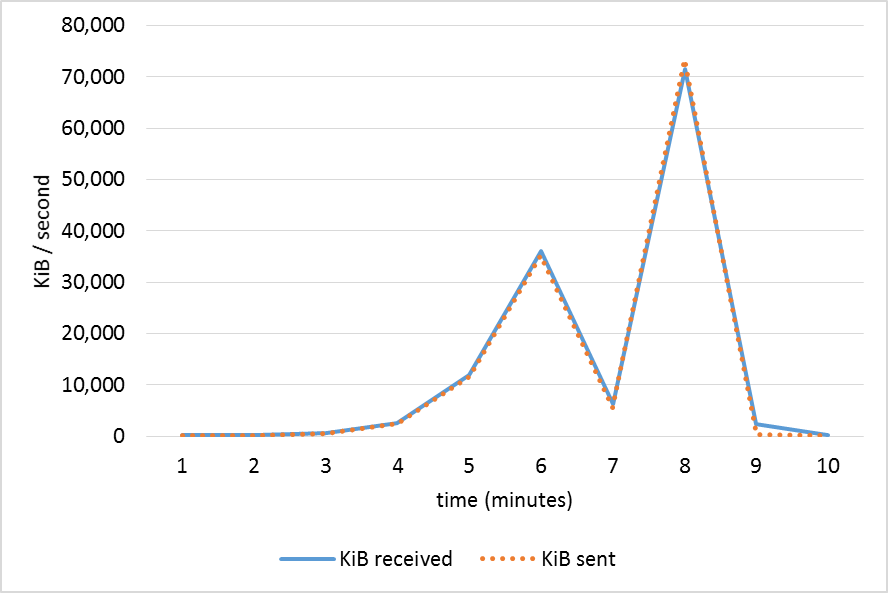
\includegraphics[width=5in]{immagini_extension/comm_cost_pems.png}
\caption{Received and sent data in the commodity cluster network during PEMS-SF dataset mining, minsup=20.}
\label{comm_cost_pems}
\end{figure}

\begin{figure}[!t]
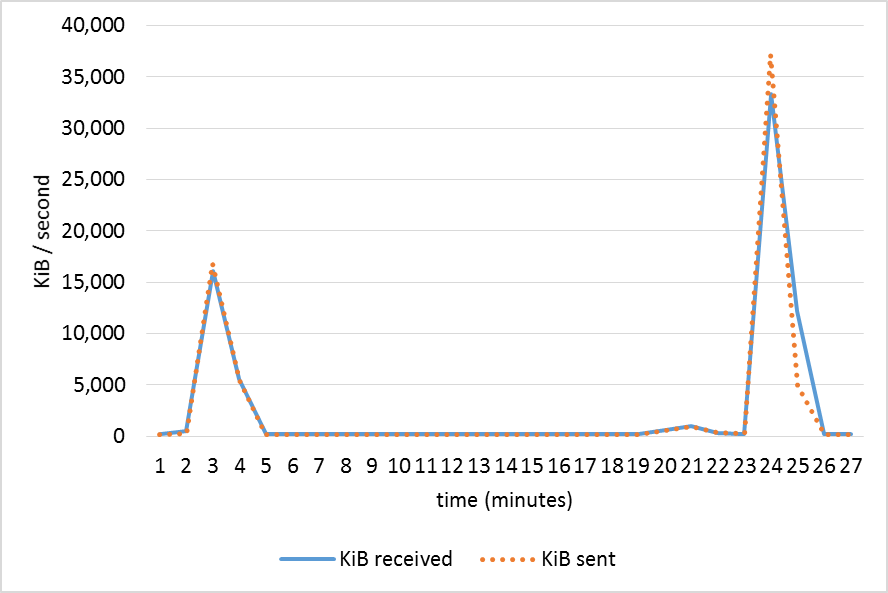
\includegraphics[width=5in]{immagini_extension/comm_cost_breast.png}
\caption{Received and sent data in the commodity cluster network during Breast Cancer dataset mining, minsup=6.}
\label{comm_cost_breast}
\end{figure}

The load balancing is evaluated comparing the execution time of the fastest and slowest tasks related to the iteration job in which this difference is strongest. The most unbalanced phase of the job is, not surprisingly, the mapper phase of the Job 3. This job is iterated until the mining is complete and it is the one more involved by the increasing of increasing of the $max\_exp$ parameter (iterations characterized by high $max\_exp$ value are likely characterized by long and unbalanced task).
\begin{table}
\begin{center}
\caption{Load Balancing}
\label{load balance final}
\begin{tabular}{ | c | c| c| }
\hline
	Dataset						    & Slowest Task & Fastest Task  \\
							    &  Execution time &  Execution time \\ \hline \hline
	PEMS-SF & 3mins 58 sec & 3mins 37sec \\ \hline
	Breast Cancer & 20mins 33sec & 8mins 42sec\\ \hline
%\multicolumn{2}{|c|}{Task execution time}    & \multicolumn{2}{|c|}{Task execution time}      \\ 
% & \multicolumn{2}{|c|}{Breast Cancer}    & \multicolumn{2}{|c|}{PEMS-SF}      \\ \hline
%	Maximum expansion threshold &   Min          & Max    &   Min          & Max          \\ \hline
%	100,000,000                 &    7 m                      & 2h 16m 17s &    44s                      & 2h 20m 28s
%  \\ \hline
%10                         &    6m 21s                      &        45m 16s  &   6s                      &        2m 24s
% \\ \hline
\end{tabular}
\end{center}
\end{table}
The difference among the fastest and the slowest mapper, as shown by Table~\ref{load balance final}. It is clear that the mining on PEMS-SF dataset is more balanced among the independent tasks. Even in this case, the reason is the different increment value in the Strategy \#1 (10 for PEMS-SF dataset, 10,000 for Breast Cancer dataset). A slower $max\_exp$ increasing leads to more balanced tasks.


%The difference among the fastest and the slowest mapper, as shown by Table~\ref{load balance final}, is not negligible. However, for both the datasets mining, the most unbalanced job is in a phase of the global mining in which there are a lot of input data, which correspond to a number of HDFS chunk greater than the number of mapper. Therefore, even if a long-tailed job does happen, the commodity cluster resources are not completely wasted because new mappers are scheduled as soon as the first ones are processed. This mitigates the load unbalance and the resource lose.




%This section addresses the scalability of PaMPa-HD with respect to the
%number of reducers, since the most heavy operations (i.e.,
%the execution of the ``local'' Carpenter) are executed by the reducers.
%The number of reducers varies from 1 to 18, 
%which is the maximum number of tasks that can be run simultaneously 
%in the commodity cluster at our disposal.
%The Breast cancer dataset and a minimum absolute
%support threshold equal to 6 have been used.
%As shown in figure~\ref{scalability}, 
%the increase of the number of reducers has
%a positive impact on the execution time
%when the number of reducers is less than 10.
%The marginal benefits decrease as more reducers are added to the computation.
%Therefore, with more than 10 reducers, the benefits of the load distribution
%are compensated by the decreased effectiveness of the local pruning (i.e., the
%more the load is distributed, the less effective the local pruning is).
% %As already mentioned, the behavior is strictly connected with the considered
% dataset.

%
%\begin{figure}[!t]
%\includegraphics[width=5in]{grafo_scalability.png}
%\caption{Execution time with different numbers of reducers on Breast Cancer dataset with $minsup$=6.}
%\label{scalability}
%\end{figure}

